\section{Introduction}
\seclabel{introduction}

With ``Cloud Robotics and Automation," systems exchange data and perform computation via networks instead of operating in isolation with limited computation and memory.
Potential advantages to using the Cloud include Big Data, or access to updated libraries of images, maps, and object/product data, and Cloud Computing, or access to parallel grid computing for statistical analysis, machine learning, and planning.
Similar advantages have recently been used for vision and speech, where datasets with millions of examples such as ImageNet~\cite{deng2009imagenet} and the Fisher corpus~\cite{cieri2004fisher} have produced results~\cite{hannun2014deepspeech, hays2008im2gps, krizhevsky2012imagenet} that surpass those obtained from decades of research on analytic methods~\cite{kehoe2015survey}.
This suggests that large-scale machine learning of grasps for vast numbers of possible object shapes, object poses, environment configurations, etc.~\cite{goldfeder2011data, lenz2015deep, kappler2015leveraging}, could exhibit scaling effects similar to those observed in computer vision and speech recognition.

\begin{figure}[t!]
\centering
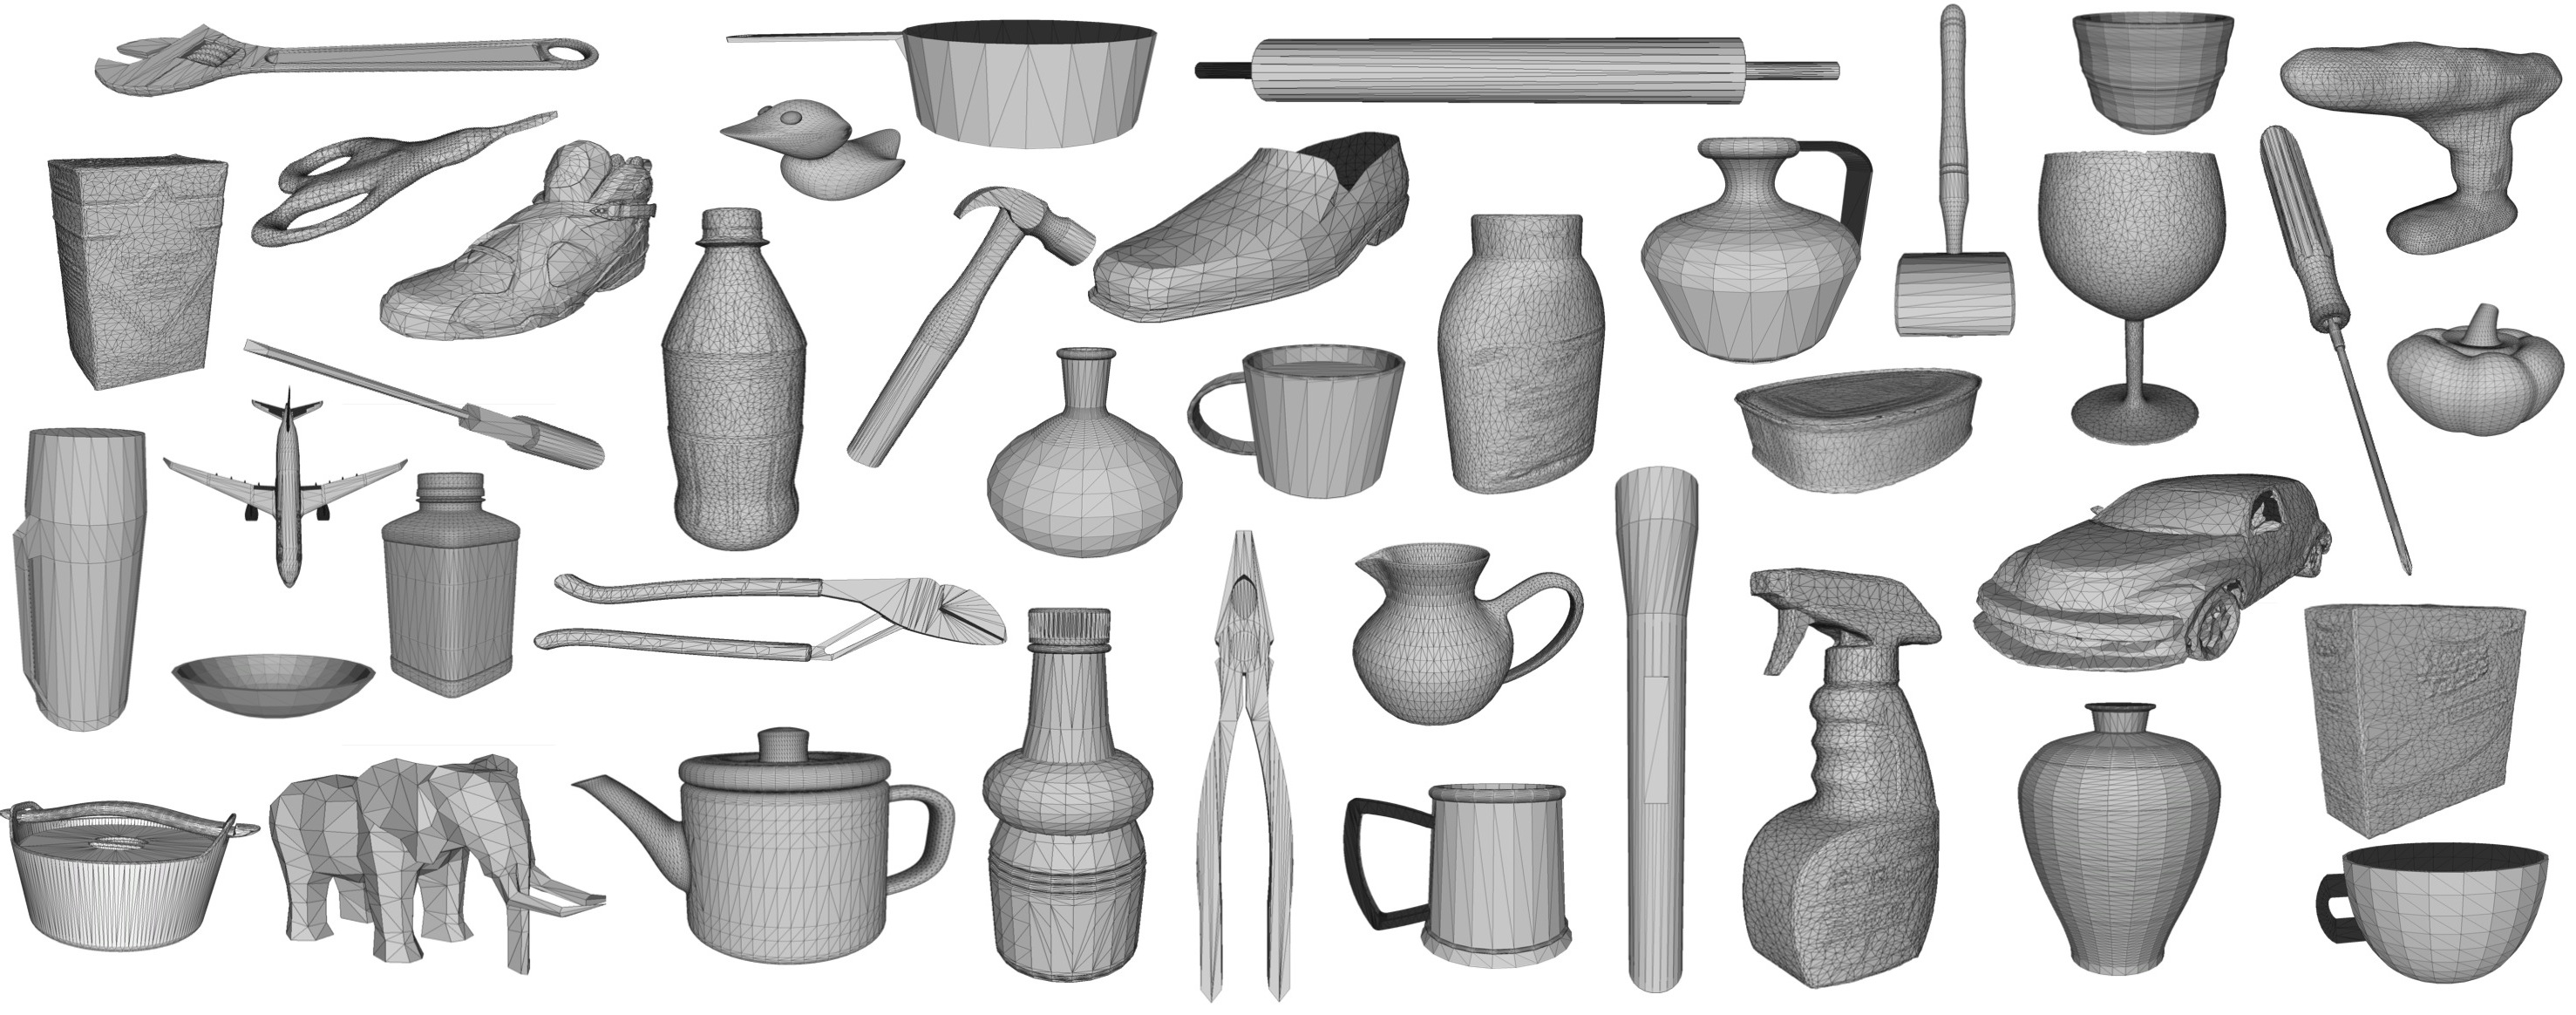
\includegraphics[scale=0.085]{figures/dexnet_collage.jpg}
\caption{Sample of 3D mesh models from the Dex-Net dataset that currently includes over 10,000 models from the KIT object database~\cite{kasper2012kit}, the Yale-CMU-Berkeley object set~\cite{calli2015benchmarking}, 3DNet\cite{wohlkinger20123dnet}, ModelNet~\cite{wu20143d}, and the SHREC 2014 object retrieval challenge dataset~\cite{li2015comparison}. }
\figlabel{dexnet-teaser}
\vspace*{-15pt}
\end{figure}

Our primary contribution is a Multi-Armed Bandit (MAB) algorithm with correlated rewards to scale robust planning by learning from a large dataset of prior grasps and 3D object models.
Our algorithm is based on Continuous Correlated Beta Processes (CCBPs)~\cite{goetschalckx2011continuous, montesano2012active}, an efficient model for predicting a belief distribution on the quality of each grasp from prior data.

To study scaling effects we develop Dex-Net 1.0, a growing dataset othat currently includes over 10,000 3D object models scaled to fit within a PR2 gripper and selected to reflect objects that could be encountered in warehousing or the home such as containers, tools, tableware, and toys.
~\figref{dexnet-teaser} shows a sample of the objects in the dataset.
%Dex-Net contains laser-scanned 3D mesh models from the KIT object database~\cite{kasper2012kit}, the Amazon Picking Challenge objects, BigBIRD~\cite{singh2014bigbird}, and YCB~\cite{calli2015benchmarking} to reflect physical objects commonly used for benchmarking in grasping research.
%The dataset also includes synthetic 3D mesh models from shape classification datasets such as 3DNet~\cite{wohlkinger20123dnet}, ModelNet~\cite{wu20143d}, and the SHREC 2014 large scale object retrieval challenge~\cite{li2015comparison} to approach larger scales.
Dex-Net also contains approximately 2.5 million parallel-jaw grasps, as each object is labelled with up to 250 grasps and an estimate of the probability of force closure for each under uncertainty in object pose, gripper pose, and friction coefficient.
To the best of our knowledge, this is the largest dataset used for grasping research to-date.
We also incorporate multi-view Convolutional Neural Networks (MV-CNNs)~\cite{su2015multi}, a state-of-the-art method for 3D shape classification, to efficiently retrieve similar 3D objects. 

We implement our algorithm on Google Compute Engine and store Dex-Net 1.0 on Google Cloud Storage, with a system that can run up to 1,500 instances at once.
Experiments on planning parallel-jaw grasps with high probability of force closure with our algorithm suggest that using 10,000 prior object models from Dex-Net can reduce the average number of samples needed to identify a grasp with high quality by $3.5\times$.
\TODO{Update with final results}

 





